\section{GPUs}\label{sec:gpus}
\mkAgenda
\begin{frame}{GPUs}
    \begin{columns}
        \begin{column}{0.4\textwidth}
            \begin{itemize}
                \item<1-> Originally: accelerate graphics (for games)
                \item<2-> Programmable shaders: flexibility
                \item<3-> Much more performant than CPUs
                \item<4-> General purpose (CUDA, 2007)
            \end{itemize}
        \end{column}

        \begin{column}{0.5\textwidth}
            \includegraphics<1-2>[width=0.7\linewidth]{./figures/geforce_256}
            \includegraphics<1-2>[width=0.7\linewidth]{./figures/rtx4090}
            \onslide*<3>{\resizebox{0.9\linewidth}{!}{\input{./figures/time.pgf}}}
            \includegraphics<4>[width=0.9\linewidth]{./figures/applications}
        \end{column}
    \end{columns}
\end{frame}

\begin{frame}{GPUs}
    \center
    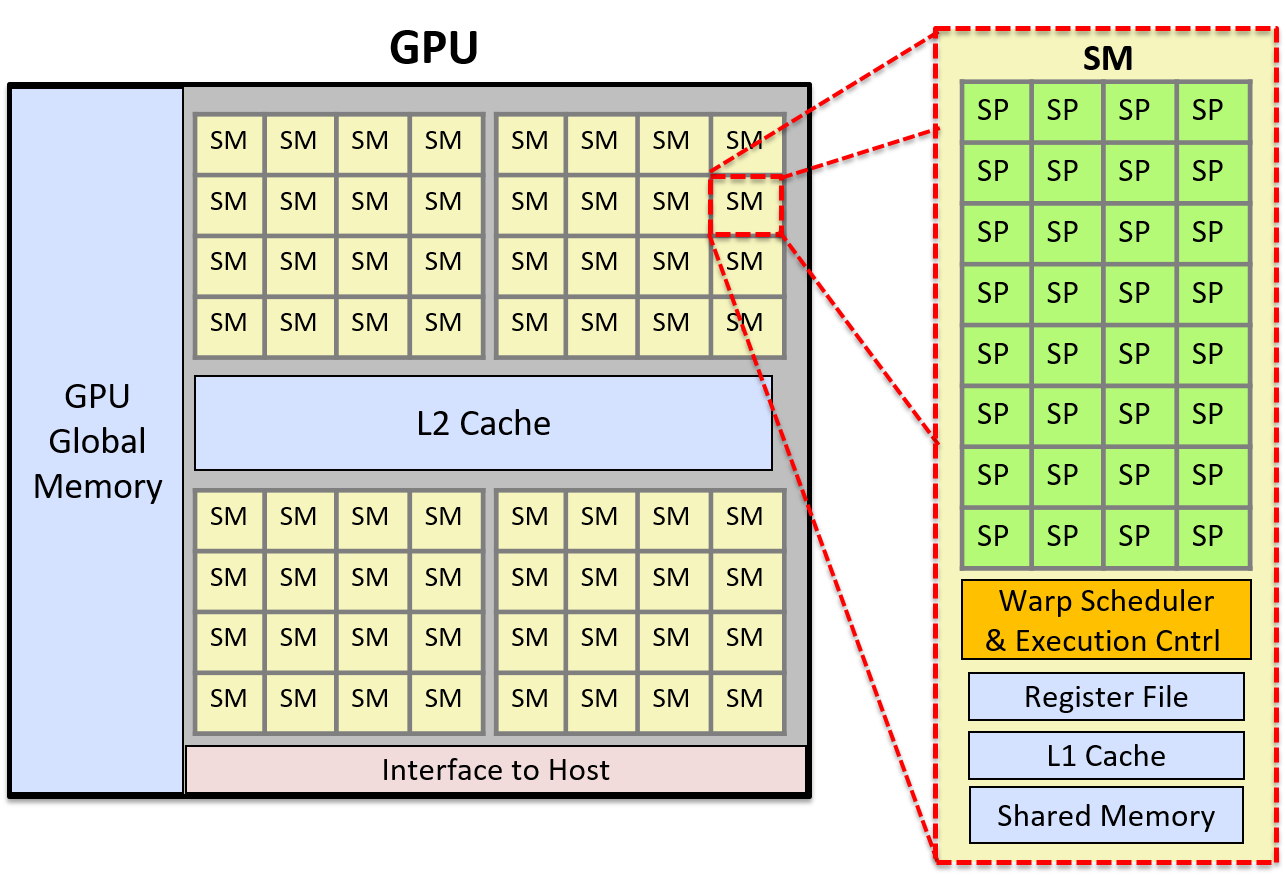
\includegraphics[width=0.45\linewidth]{./figures/arch}
    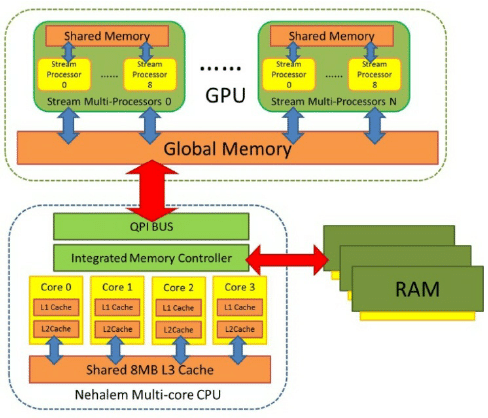
\includegraphics[width=0.45\linewidth]{./figures/interaction}
\end{frame}